The objectives of this experiment are to familiarise ourself with epicyclic gearing system and experimentally analytically determine the velocity ratios of epicyclic gear system by making the carrier arm, annulus gear, and sun gear fixed one at a time. The apparatus for this experiment consists of four gears as seen on the image below and individual shafts are able to be locked independently in order for us to carry the experiment. \\
\begin{figure}[H]
\centering
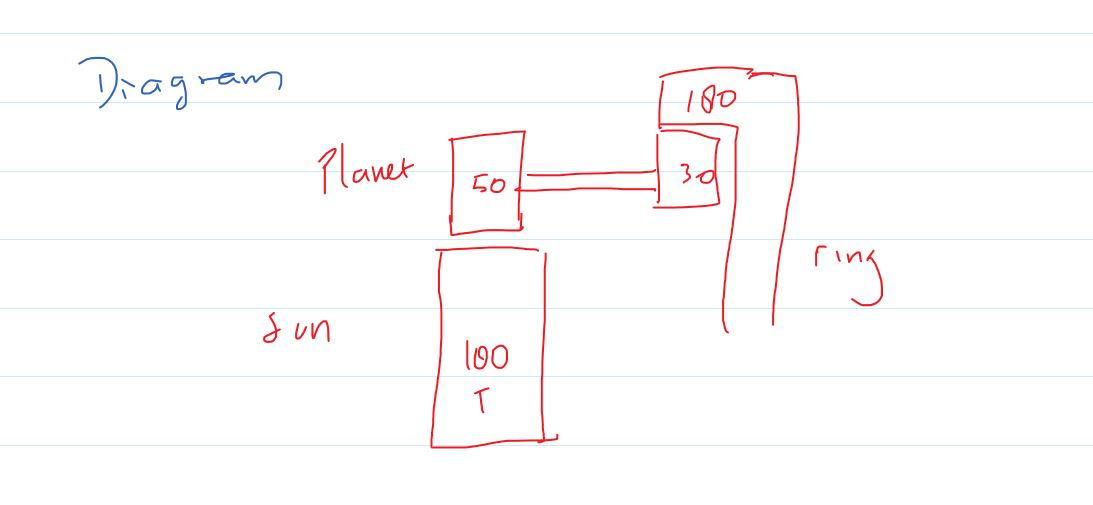
\includegraphics[width=1\textwidth]{chapters/lab3/geardrawing}
\caption{Epicyclic gear drawing.}
\label{fig:mesh1}
\end{figure}
This experiment is divided into three parts with the first part is to determine the speed ratio between the input shaft (sun gear) and the output shaft (annulus gear). The second part also to determine the velocity ratio between input and output shafts (sun and the carrier arm) with the annulus or ring gear is fixed. The last part is to determine the velocity ratio between the carrier arm (input) and the annulus gear or the ring gear (output). However, in this part, the sun gear is fixed. \\

In this experiment the constants are the number of teeth and it is shown below:
\begin{itemize}
\item $T_{sun}$ = 100 Teeth.
\item $T_{planet_1}$ = 50 Teeth.
\item $T_{planet_2}$ = 30 Teeth.
\item $T_{ring}$ = 180 Teeth.
\end{itemize}
Where $T_{planet_1}$ is the planet gear that is meshing to the sun gear and $T_{planet_2}$ is the planet gear that is meshing with the ring gear.